% ===============================================================
\section{Results and Discussion}\label{sec:results}
% ===============================================================

\subsection{RQ1: End-to-end Answer Quality}\label{subsec:rq1}

Since the ultimate purpose of routing is to produce better answers, we first
ask whether adaptive routing improves end-to-end quality over fixed-strategy
baselines, and whether Stage~2 contributes beyond correcting route selection.
Two ablations isolate the mechanisms: an Oracle Router that dispatches every
query using its gold route label without Stage~2, and an
\textit{Oracle~+~Stage~2} configuration that holds routing at gold labels
while enabling the verifier, so that any difference between the two is
attributable to Stage~2 reasoning alone. Table~\ref{tab:end_to_end} reports
results on the strict $600$-query benchmark with bootstrap $95\%$ confidence
intervals ($B=1000$, seed~$42$), and Fig.~\ref{fig:f1_bar} visualises
Answer~F1 across the six main systems.

% NOTE(M6): the BERT-F1 column is still \pending -- running BERTScore over the
% saved predictions (run_full_eval --bert) is a submission blocker.
% NOTE: the Always-on S2 trigger rate is \pending because the logged rate
% (79.5%) contradicts the definition of the configuration (must be 100%);
% verify from full_eval_log.jsonl whether the always_invoke_stage2 flag was
% actually bound (HybridPipeline silently retries WITHOUT kwargs it rejects)
% and re-run if not. Until resolved, treat the Always-on row as provisional.
\begin{table*}[!htbp]
\centering
\caption{End-to-end results on the strict $600$-query Vietnamese legal QA
benchmark. Route~Acc is the agreement between the \emph{executed} route and
the gold label, measured after Stage-2 overrides, clarification decisions,
and execution-time fallbacks. F1 and EM are token-level scores from
\texttt{evaluate\_prediction}, with bootstrap $95\%$ confidence intervals in
brackets; BERT-F1 is the semantic complement
(Section~\ref{subsec:metrics}). Hit@$1$ uses canonical identifier matching in
strict mode. S2 is the Stage~2 trigger rate. Bold marks the best value per
column, excluding the two oracle rows}\label{tab:end_to_end}
\small
\begin{tabular}{lrlrcrrr}
\toprule
\textbf{System} & \textbf{Route Acc} & \textbf{F1 {\scriptsize[95\% CI]}} & \textbf{EM} & \textbf{BERT-F1} & \textbf{Hit@1} & \textbf{Lat (ms)} & \textbf{S2} \\
\midrule
Pure Vector  & 0.500 & \textbf{0.663} {\scriptsize[0.635, 0.690]} & 0.152 & \pending & \textbf{0.727} & 14{,}241 & -- \\
Pure Graph   & 0.250 & 0.633 {\scriptsize[0.607, 0.659]} & \textbf{0.335} & \pending & 0.545 & \textbf{9{,}530} & -- \\
Pure Hybrid  & 0.250 & 0.661 {\scriptsize[0.637, 0.681]} & 0.108 & \pending & 0.003 & 10{,}766 & -- \\
Single-stage & \textbf{0.732} & 0.475 {\scriptsize[0.447, 0.502]} & 0.132 & \pending & 0.365 & 9{,}711 & 0.0\% \\
Two-stage (ours) & 0.667 & 0.640 {\scriptsize[0.618, 0.666]} & 0.260 & \pending & 0.000$^{\dag}$ & 10{,}324 & 79.5\% \\
Always-on Stage~2 & 0.667 & 0.645 {\scriptsize[0.621, 0.669]} & 0.258 & \pending & 0.000$^{\dag}$ & 10{,}047 & \pending \\
\midrule
Oracle       & 1.000 & 0.563 {\scriptsize[0.538, 0.590]} & 0.157 & \pending & 0.000$^{\dag}$ & 7{,}862 & -- \\
Oracle + Stage~2 & 0.670 & 0.637 {\scriptsize[0.614, 0.661]} & 0.243 & \pending & 0.000$^{\dag}$ & 9{,}992 & 79.5\% \\
\bottomrule
\multicolumn{8}{l}{\footnotesize $^{\dag}$Measured value reflects logged
source identifiers that the canonical normaliser cannot resolve for
router-mediated}\\
\multicolumn{8}{l}{\footnotesize \phantom{$^{\dag}$}configurations, not true
coverage; the retrieval-stage identifier fix and re-run are pending
(Section~\ref{sec:limitations}).}\\
\end{tabular}
\end{table*}

\begin{figure}[!htbp]
\centering
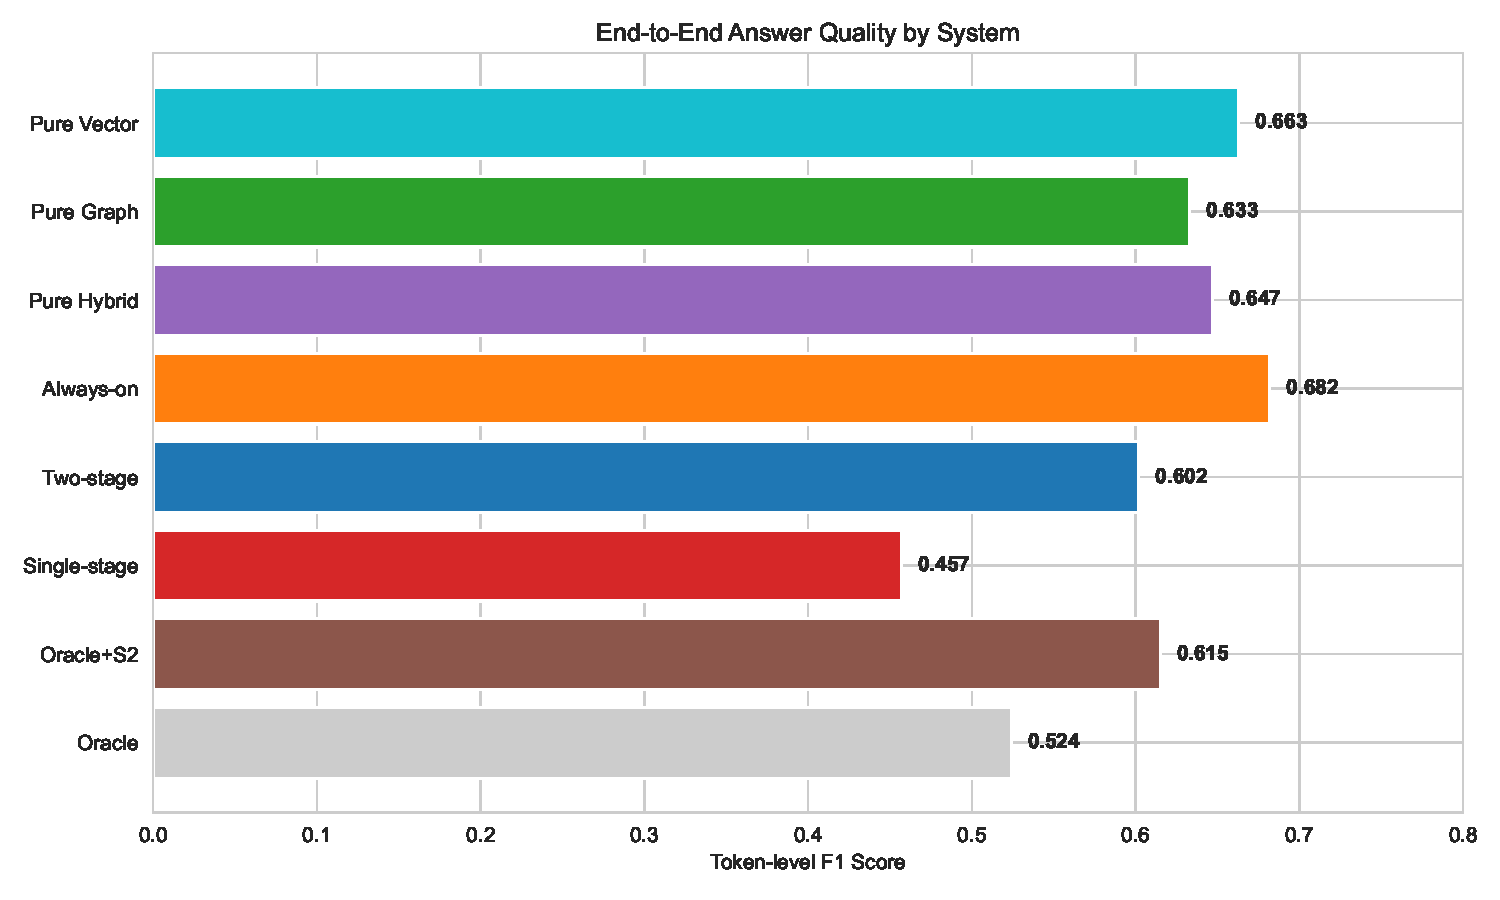
\includegraphics[width=\columnwidth]{figs/f1_bar.pdf}
\caption{Answer~F1 on the strict $600$-query benchmark with bootstrap $95\%$
confidence intervals. Pure Vector is the strongest fixed-strategy baseline
($0.663$); the Two-stage Router ($0.640$) is statistically indistinguishable
from it and outperforms the Oracle ($0.563$), while the Single-stage Router
($0.475$) is the weakest, underscoring the role of
Stage~2}\label{fig:f1_bar}
\end{figure}

We make the following observations.

\noindent\textbf{Stage~2 reasoning causally improves answers.} The
\textit{Oracle~+~Stage~2} configuration reaches F1~$=0.637$
{\scriptsize[$0.614, 0.661$]} against F1~$=0.563$
{\scriptsize[$0.538, 0.590$]} for the plain Oracle---a $+0.074$ gain with
\emph{non-overlapping} confidence intervals under \emph{identical} gold
routing. Because routing is held fixed, this difference is attributable to
Stage~2's explicit reasoning over query intent and legal constraints during
verification and generation, confirming the chain-of-thought interpretation
that the earlier Two-stage$\,>\,$Oracle contrast ($0.640$ vs $0.563$,
$+0.077$, also CI-separated) could only suggest.

\noindent\textbf{Stage~2 accounts for the routing-to-quality gain.} The gap
between the Single-stage Router (F1~$=0.475$) and the Two-stage Hybrid
(F1~$=0.640$) is $+0.165$ with non-overlapping intervals. Because the two
systems share an identical Stage~1, this entire gap is attributable to
selective Stage~2 verification.

\noindent\textbf{Better answers, not better route agreement.} Executed-route
accuracy actually \emph{drops} from the Single-stage Router ($0.732$) to the
Two-stage Hybrid ($0.667$), and even Oracle~+~Stage~2 retains only $0.670$
agreement with the gold labels because the verifier overrides them---yet F1
rises in both cases. Stage~2's value therefore lies in reasoning during
answer generation rather than in reproducing the gold routing taxonomy, which
is precisely the chain-of-thought behaviour claimed.

\noindent\textbf{Selective invocation matches always-on verification.} The
Two-stage Hybrid ($0.640$ {\scriptsize[$0.618, 0.666$]}) is statistically
indistinguishable from Always-on Stage~2 ($0.645$
{\scriptsize[$0.621, 0.669$]}), so triggering the verifier on $79.5\%$ of
queries retains the quality of unconditional verification
(Section~\ref{subsec:rq4} analyses the trigger policy).

\noindent\textbf{The router matches, but does not surpass, the strongest
fixed baseline on aggregate token-F1.} Pure Vector attains the highest
fixed-strategy F1 ($0.663$ {\scriptsize[$0.635, 0.690$]}) and coverage
(Hit@$1=0.727$ {\scriptsize[$0.692, 0.763$]}); the Two-stage router
($0.640$ {\scriptsize[$0.618, 0.666$]}) overlaps this interval and is
therefore statistically indistinguishable from it on this dense-dominated
distribution. The router's advantages lie elsewhere: exact match is $71\%$
higher than Pure Vector ($0.260$ vs $0.152$), the highest EM of any
non-fixed configuration; and, unlike any fixed strategy, the router can
refuse to guess by clarifying (Section~\ref{subsec:rq3}).

\noindent\textbf{Pure Graph trades fluency for relational precision.} It
reaches the highest EM overall ($0.335$) but a lower F1 ($0.633$), reflecting
concise answers generated from highly structured graph context.

\noindent\textbf{Pure Hybrid exposes a residual engineering gap.} Its
retrieval coverage collapses to near zero (Hit@$1=0.003$) because the hybrid
merge path emits source identifiers that the canonical normaliser cannot
resolve to the gold scheme; the router-mediated configurations inherit the
same logging defect (the $\dag$ rows), so their Hit@$1$ values understate
true coverage pending the retrieval-stage fix
(Section~\ref{sec:limitations}).

To locate \emph{where} each system earns its score,
Table~\ref{tab:per_class_f1} reports Answer~F1 separately by gold routing
class.

\begin{table}[!htbp]
\centering
\caption{Answer~F1 broken down by gold routing class on the strict benchmark
($300$ dense / $150$ graph / $150$ hybrid queries). Bold marks the best value
per column}\label{tab:per_class_f1}
\begin{tabular}{lrrr}
\toprule
\textbf{System} & \textbf{Dense F1} & \textbf{Graph F1} & \textbf{Hybrid F1} \\
\midrule
Pure Vector      & 0.549 & \textbf{0.888} & \textbf{0.667} \\
Pure Graph       & \textbf{0.810} & 0.499 & 0.415 \\
Pure Hybrid      & 0.605 & 0.801 & 0.631 \\
Single-stage     & 0.596 & 0.373 & 0.333 \\
Two-stage (ours) & 0.676 & 0.592 & 0.618 \\
Always-on Stage~2 & 0.677 & 0.597 & 0.630 \\
\midrule
Oracle           & 0.519 & 0.588 & 0.625 \\
Oracle + Stage~2 & 0.669 & 0.584 & 0.625 \\
\bottomrule
\end{tabular}
\end{table}

The per-class pattern is striking and initially counter-intuitive:
\emph{each pure mechanism scores highest on the other mechanism's class}.
Pure Graph attains the best F1 on dense-class queries ($0.810$) while Pure
Vector attains the best F1 on graph-class queries ($0.888$). The class-wise
means are internally consistent with the aggregate column of
Table~\ref{tab:end_to_end} under the $300{:}150{:}150$ class weights, so
this is a genuine property of the measurements, not a tabulation error. We
interpret it as a metric--prompt interaction rather than as evidence about
mechanism appropriateness: token-F1 is computed against a gold context, and
the citation-constrained generator quotes legal text verbatim, so a system
scores highly on a class whenever it happens to quote text with high lexical
overlap with that class's gold contexts---graph-class gold contexts are
article passages that dense retrieval reproduces nearly verbatim whenever the
target article is findable by embedding similarity, while concise dense-class
factoid questions penalise over-quotation. Exact match, which is insensitive
to quotation length, shows the expected mechanism alignment (Pure Graph
attains the highest EM, driven by relation-heavy queries). The consequence is
methodological: \emph{per-class token-F1 cannot adjudicate which retrieval
mechanism suits which query class}, which is why the semantic BERT-F1 column
of Table~\ref{tab:end_to_end} is a required complement rather than an
optional extra (Section~\ref{subsec:metrics}). What the per-class table does
establish is the router's balance and the locus of Stage~2's contribution:
the Two-stage system has the most even non-oracle profile
($0.676/0.592/0.618$), and its gains over the Single-stage Router are
concentrated exactly on the graph-class ($+0.219$) and hybrid-class
($+0.285$) queries where Stage~1 alone collapses.

\subsection{RQ2: Routing Accuracy}\label{subsec:rq2}

A router is useful only if it selects the correct retrieval mechanism. We
evaluate routing from two complementary angles: the generalisation of the
deployed router on the paraphrase-hardened strict test split, and a
controlled comparison of classifier families under one identical
cross-validation protocol on the training data.

\paragraph{Generalisation on the strict split.}
Table~\ref{tab:routing_strict} reports the routing decision of the deployed
two-stage router on the $600$ strict test queries, whose surface templates
were paraphrased away from the training distribution. The router attains
$0.898$ overall accuracy and $0.900$ macro-F1 over the three retrieval
classes, with its weakest precision on the graph class ($0.790$), where
dense-class queries occasionally carry incidental relation cues. It
additionally emitted nine clarification requests ($1.5\%$) on answerable
queries---the only clarify false positives observed on this split.
% NOTE: P and F1 in this table are derived arithmetically from the reported
% confusion counts (prediction distribution per gold class). The offline
% routing pass recorded a Stage-2 trigger rate of 55.8%, which differs from
% the 79.5% observed end-to-end -- reconcile (likely different tau_conf or
% feature context between the offline sanity run and the live pipeline)
% before submission.

\begin{table}[!htbp]
\centering
\caption{Deployed router on the strict $600$-query split: per-class recall
(R), precision (P), and F1 over the three retrieval classes. Overall accuracy
$0.898$; macro-F1 $0.900$. Nine clarify decisions ($1.5\%$) were emitted on
answerable queries}\label{tab:routing_strict}
\begin{tabular}{lrrrr}
\toprule
\textbf{Gold class} & \textbf{N} & \textbf{R} & \textbf{P} & \textbf{F1} \\
\midrule
Dense retrieval  & 300 & 0.890 & 0.964 & 0.926 \\
Graph traversal  & 150 & 0.853 & 0.790 & 0.820 \\
Hybrid reasoning & 150 & 0.960 & 0.947 & 0.953 \\
\midrule
\textbf{Overall / macro} & 600 & 0.901 & 0.900 & 0.900 \\
\bottomrule
\end{tabular}
\end{table}

\paragraph{Classifier comparison under identical cross-validation.}
Table~\ref{tab:routing_cv} compares six classifiers under one stratified
five-fold protocol (identical folds, seed~$42$) over the $860$ training
samples ($800$ routing-labelled queries plus $60$ synthetic \texttt{clarify}
samples). Learned classifiers dominate the heuristic baselines by a wide
margin---at least $0.37$ accuracy and $0.44$ macro-F1 separate the weakest
learned model from the strongest rule-based one---confirming that routing
among evidence mechanisms cannot be reduced to a handful of surface rules.

\begin{table}[!htbp]
\centering
\caption{Routing classifiers under identical stratified five-fold
cross-validation on the training data (mean\,$\pm$\,std across folds).
Absolute values for the learned models are optimistic due to pre-split
paraphrase leakage (see text); the deployment-relevant figure is the
strict-split result of Table~\ref{tab:routing_strict}}\label{tab:routing_cv}
\begin{tabular}{lrr}
\toprule
\textbf{Classifier} & \textbf{CV Acc.} & \textbf{CV Macro-F1} \\
\midrule
Majority Route        & $0.4651\ \ci{0.0000}$ & $0.1587\ \ci{0.0000}$ \\
Keyword Rule Router   & $0.6081\ \ci{0.0182}$ & $0.3866\ \ci{0.0263}$ \\
Simple 3-Rule Router  & $0.6209\ \ci{0.0222}$ & $0.5422\ \ci{0.0308}$ \\
Logistic Regression   & $0.9953\ \ci{0.0044}$ & $0.9953\ \ci{0.0042}$ \\
Random Forest         & $0.9965\ \ci{0.0028}$ & $0.9966\ \ci{0.0029}$ \\
XGBoost (Stage~1, deployed) & $0.9942\ \ci{0.0037}$ & $0.9944\ \ci{0.0035}$ \\
\bottomrule
\end{tabular}
\end{table}

\paragraph{Leakage analysis: reconciling the routing figures.}
All three learned models exceed $0.99$ under cross-validation, which a
quantitative leakage analysis shows to be optimistic: because paraphrase
augmentation was applied \emph{before} splitting, $33.2\%$ of highly similar
query pairs (token Jaccard $\ge 0.7$) straddle the fold boundary, and the
mean Jaccard similarity of cross-fold pairs ($0.192$) is essentially equal to
that of within-fold pairs ($0.190$)---the folds do not isolate query
templates, so every learned model partially recognises test templates from
training. This resolves the apparent conflict between the routing figures
reported at different points of this project: the single-split and
cross-validated results ($\approx 0.99$) share the same template leakage and
should be read as upper bounds on separability given the features, whereas
the strict-split accuracy of $0.898$
(Table~\ref{tab:routing_strict})---measured on paraphrase-hardened queries
disjoint from training---is the honest generalisation estimate and the figure
we headline. Constructing template-grouped folds is left as an evaluation
improvement for future work.

\noindent\textbf{Feature reliance and efficiency.} The decision is driven
mainly by structural signals---the legal reference count, query length,
cross-document signals, and article reference count---rather than by spurious
lexical artefacts (Section~\ref{subsec:features};
Appendix~\ref{app:repro}, Table~\ref{tab:features}). The classifier forward
pass takes $\approx\!8.9$~ms on CPU versus $\approx\!53.3$~ms on GPU for a
PhoBERT classifier, making Stage~1 well suited to gating the expensive
Stage~2 verifier; the decisive evidence for the design, however, is the
end-to-end quality and latency trade-off of RQ1 and RQ5.

\subsection{RQ3: Ambiguity and Clarification Handling}\label{subsec:rq3}

Routing is safety-critical when the legal target is underspecified: retrieving
against an arbitrary document yields a confidently wrong answer. We evaluate
the deployed system on the $234$-query ambiguity benchmark ($156$ ambiguous
queries, $78$ answerable controls) and on the $160$-query multi-turn
conversation stress test ($8$ scenario types $\times$ $20$ dialogues).
Table~\ref{tab:ambiguity} summarises both benchmarks;
Table~\ref{tab:ambiguity_type} breaks the conversation results down by
scenario type.

\begin{table}[!htbp]
\centering
\caption{Clarification performance of the deployed router. P, R, and F1 are
computed over the \texttt{clarify} decision against the binary
ambiguous/answerable gold label; Overr.\ is the rate at which Stage~2
overrides the Stage~1 proposal}\label{tab:ambiguity}
\small
\begin{tabular}{lrrrrrr}
\toprule
\textbf{Benchmark} & \textbf{Route Acc.} & \textbf{P} & \textbf{R} & \textbf{F1} & \textbf{S2 Trig.} & \textbf{S2 Overr.} \\
\midrule
Ambiguity ($N{=}234$)    & 0.761 & 0.945 & \textbf{1.000} & \textbf{0.972} & 85.0\% & 5.5\% \\
Conversation ($N{=}160$) & 0.725 & 0.857 & 0.960 & 0.906 & 91.9\% & 13.6\% \\
\bottomrule
\end{tabular}
\end{table}

\begin{table}[!htbp]
\centering
\caption{Conversation stress test by scenario type ($20$ dialogues each).
Clarify F1 is $0.000$ by construction for scenario types whose gold label is
a retrieval route rather than \texttt{clarify}}\label{tab:ambiguity_type}
\small
\begin{tabular}{lrrr}
\toprule
\textbf{Scenario type} & \textbf{Route Acc.} & \textbf{Clarify F1} & \textbf{S2 Trig.} \\
\midrule
Clarify, no history          & 1.000 & 1.000 & 1.00 \\
Missing entity               & 1.000 & 1.000 & 1.00 \\
Multi-interpretation         & 1.000 & 1.000 & 1.00 \\
Irrelevant history           & 0.950 & 0.974 & 0.95 \\
Conflicting history          & 0.850 & 0.919 & 0.90 \\
Answerable with history      & 0.500 & 0.000 & 0.85 \\
Clear graph/hybrid (control) & 0.400 & 0.000 & 0.75 \\
Clear dense (control)        & 0.100 & 0.000 & 0.90 \\
\bottomrule
\end{tabular}
\end{table}

We make the following observations.

\noindent\textbf{Every ambiguous query is intercepted.} On the ambiguity
benchmark the router attains clarify recall $1.000$ at precision $0.945$
(F1~$=0.972$): none of the $156$ ambiguous queries reaches retrieval, at the
cost of spuriously clarifying roughly nine of the $78$ answerable controls
($11.5\%$). For a legal assistant this operating point is the safer side of
the trade---a missed ambiguity produces a confidently wrong answer grounded
in the wrong document, whereas a spurious clarification costs a single
dialogue turn. The contrast between the $11.5\%$ false-positive rate on the
diagnostic's controls and the $1.5\%$ clarify rate on the ambiguity-free
strict split (Section~\ref{subsec:rq2}) shows, however, that precision
degrades as the ambiguity base rate of the surrounding traffic rises.

\noindent\textbf{Semantic underspecification is detected, not just surface
cues.} The two scenario types that carry no surface marker of
ambiguity---missing entity and multi-interpretation, where the query is
grammatically complete but legally underdetermined---are detected perfectly
(clarify F1~$=1.000$, trigger rate $100\%$). The indicator families targeting
generic legal needs without a concrete anchor ($\psi_6$) and broad
subject--predicate combinations without a domain anchor ($\psi_8$), combined
with the weakly supervised Stage~1 clarify class, therefore capture semantic
underspecification rather than merely pronoun surface cues.

\noindent\textbf{History conditions are handled asymmetrically.} Dialogues
whose history is irrelevant or conflicting are clarified near-perfectly
(F1~$=0.974$ and $0.919$), and clarification without history is perfect. The
weak case is \emph{answerable with history}: only half of the queries whose
referent the resolver can recover are subsequently routed to the correct
retrieval mechanism, the remainder being either spuriously clarified or
dispatched to the wrong route.

\noindent\textbf{Clear queries embedded in conversation are misrouted.} The
two control scenario types expose the principal remaining weakness:
self-contained dense queries inside a dialogue are routed correctly only
$10\%$ of the time (graph/hybrid controls: $40\%$), even though Stage~2 is
triggered on $75$--$90\%$ of them. Conversational context evidently inflates
the ambiguity and trigger signals of queries that need no context at all,
dragging them off their correct route; overall conversation route accuracy
($0.725$) is therefore bounded by control misrouting, not by clarify
detection (F1~$=0.906$). Suppressing conversational features whenever the
resolver returns \texttt{not\_needed}---that is, when the query is
self-contained---is the natural mitigation and is left to future work.

\noindent\textbf{The verifier mostly confirms Stage~1.} Stage~2 overrides its
Stage~1 proposal on only $5.5\%$ of ambiguity-benchmark queries and $13.6\%$
of conversation queries, concentrating its interventions where history must
be adjudicated. As a concrete example, given history mentioning
\textit{``Nghị định 100/2019/NĐ-CP''}, the follow-up \textit{``Văn bản đó còn
hiệu lực không?''} is resolved and routed to graph traversal, whereas with
empty history the same query is routed to \texttt{clarify}.

\subsection{RQ4: Threshold Ablation}\label{subsec:rq4}

The router exposes two key thresholds: the confidence threshold
$\tau_{\mathrm{conf}}$ that gates Stage~2, and the clarification override
threshold $\tau_{\mathrm{clar}}$. We study their effect on the development set
in Table~\ref{tab:threshold_ablation}.
% TODO (version consistency): this ablation was run on the previous system
% version; re-run scripts exist. Re-verify at least the default operating
% point after the RQ3 re-run.

\begin{table}[!htbp]
\centering
\caption{Threshold ablation on the development set}\label{tab:threshold_ablation}
\begin{tabular}{lrrr}
\toprule
\textbf{Parameter} & \textbf{Value} & \textbf{Acc.} & \textbf{S2 rate} \\
\midrule
$\tau_{\mathrm{conf}}$ & 0.50 & 0.7529 & 0.2299 \\
$\tau_{\mathrm{conf}}$ & 0.70 & 0.7529 & 0.3046 \\
$\tau_{\mathrm{conf}}$ & 0.95 & 0.7529 & 0.5920 \\
$\tau_{\mathrm{conf}}$ & 0.99 & 0.7529 & 0.5977 \\
\midrule
$\tau_{\mathrm{clar}}$ & 0.50 & 0.6839 & 0.2299 \\
$\tau_{\mathrm{clar}}$ & 0.70 & 0.7529 & 0.2299 \\
$\tau_{\mathrm{clar}}$ & 0.90 & 0.7759 & 0.2299 \\
$\tau_{\mathrm{clar}}$ & 0.95 & 0.8448 & 0.2299 \\
\bottomrule
\end{tabular}
\end{table}

We make the following observations.

\noindent\textbf{$\tau_{\mathrm{conf}}$ governs cost, not accuracy.} Sweeping
$\tau_{\mathrm{conf}}$ from $0.50$ to $0.99$ leaves routing accuracy unchanged
at $0.7529$ while raising the Stage~2 trigger rate from $0.2299$ to $0.5977$.
Many Stage~1 predictions are already high-confidence, so $\tau_{\mathrm{conf}}$
controls how much verification is spent rather than how accurate the routing
is.

\noindent\textbf{$\tau_{\mathrm{clar}}$ has a strong accuracy effect.} A low
value of $0.50$ over-clarifies on the non-ambiguous development set (accuracy
$0.6839$), whereas $0.95$ raises accuracy to $0.8448$, since a stricter
override prevents spurious clarification of answerable queries. We note that
this development-set optimum ($0.95$) differs from the default
$\tau_{\mathrm{clar}}=0.80$ used elsewhere; the two are reconciled by the
opposing pull of the two benchmarks discussed next.

\noindent\textbf{The two benchmarks pull in opposite directions.} This ablation
uses routing-oriented development data, not the ambiguity benchmark; the
$\tau_{\mathrm{clar}}$ that maximises strict routing accuracy is not the one
that maximises clarify recall, so the two objectives must be jointly calibrated
rather than tuned in isolation.

To connect this ablation to the RQ5 cost argument,
Table~\ref{tab:trigger_policy} contrasts the three verification
policies---always-off, selective (ours), and always-on---on the strict
benchmark. Selective triggering at $79.5\%$ retains the answer quality of
always-on verification ($0.640$ vs $0.645$, overlapping intervals), so the
verifier can be withheld from clearly routable queries at no measurable
quality cost.
% NOTE: the Always-on trigger-rate cell is \pending due to the 79.5%-logged
% anomaly described at Table~\ref{tab:end_to_end}; a cost comparison between
% the selective and always-on policies is deferred until that run is verified
% (the two mean latencies are within 3%, which is itself suspicious).

\begin{table}[!htbp]
\centering
\caption{Verification-policy comparison on the strict
benchmark}\label{tab:trigger_policy}
\begin{tabular}{lrrr}
\toprule
\textbf{Policy} & \textbf{S2 rate} & \textbf{F1} & \textbf{Avg lat (ms)} \\
\midrule
Always-off (Single-stage) & 0.0\%   & 0.475 & 9{,}711 \\
Selective (Two-stage, ours) & 79.5\% & 0.640 & 10{,}324 \\
Always-on & \pending & 0.645 & 10{,}047 \\
\bottomrule
\end{tabular}
\end{table}

\subsection{RQ5: Cost--Quality Trade-off}\label{subsec:rq5}

Stage~2 is powerful but expensive, so the central design question is whether
selective invocation pays off relative to always-off and always-on
verification. Table~\ref{tab:cost} reports the latency--quality analysis.
% NOTE: p50/p95 for the four re-run configurations must be extracted from
% eval_results/full_eval_log.jsonl (already logged per query by
% run_full_eval.py) -- fill the \pending cells.

\begin{table}[!htbp]
\centering
\caption{Cost--quality trade-off. S2 is the Stage~2 trigger rate; the Oracle
latency reflects gold-label routing without Stage~2 overhead}\label{tab:cost}
\small
\begin{tabular}{lrrrrr}
\toprule
\textbf{System} & \textbf{F1} & \textbf{Mean (ms)} & \textbf{p50 (ms)} & \textbf{p95 (ms)} & \textbf{S2} \\
\midrule
Pure Vector  & 0.663 & 14{,}241 & 12{,}154 & 33{,}231 & -- \\
Pure Graph   & 0.633 & \textbf{9{,}530} & \textbf{6{,}617} & 28{,}648 & -- \\
Pure Hybrid  & 0.661 & 10{,}766 & 8{,}355 & 28{,}433 & -- \\
Single-stage & 0.475 & 9{,}711 & 8{,}304 & \textbf{25{,}701} & 0.0\% \\
Two-stage (ours) & \textbf{0.640} & 10{,}324 & \pending & \pending & 79.5\% \\
Always-on Stage~2 & 0.645 & 10{,}047 & \pending & \pending & \pending \\
\midrule
Oracle       & 0.563 & 7{,}862 & \pending & \pending & -- \\
Oracle + Stage~2 & 0.637 & 9{,}992 & \pending & \pending & 79.5\% \\
\bottomrule
\end{tabular}
\end{table}

We make the following observations.

\noindent\textbf{Always-off verification is cheap but weak.} The Single-stage
Router skips Stage~2 entirely and runs at $9{,}711$~ms on average, but pays the
largest quality penalty (F1~$=0.475$); Stage~2 is the chief reason for the
$+0.165$~F1 gap to the Two-stage system.

\noindent\textbf{At the routing stage, Stage~2 is two orders of magnitude more
expensive than Stage~1.} A routing-stage microbenchmark, measured separately
from the end-to-end runs, puts one Stage~2 verifier call at
$\approx\!4{,}017$~ms against $\approx\!33.7$~ms for the full Stage~1
path---roughly a $119\times$ ratio---so unconditional verification of every
query is only viable because generation, not routing, dominates the total
budget; selective triggering remains the principled design for scaling to
higher traffic.

\noindent\textbf{End-to-end, selective verification is nearly free.} The
Two-stage system averages $10{,}324$~ms against $9{,}711$~ms for the
Single-stage Router: $+613$~ms ($+6.3\%$) buys the $+0.165$~F1 gain, because
the citation-scoped generation prompt bounds answer length and offsets much of
the verifier's cost. Against the Oracle ($7{,}862$~ms, no Stage~2), the
overhead is $\approx\!2{,}462$~ms at the $79.5\%$ trigger rate.

\noindent\textbf{Latency is dominated by generation, not by routing.} The
$\approx\!10$~s end-to-end averages dwarf the $\approx\!34$~ms Stage~1 path,
so most of the wall-clock cost is retrieval and answer generation shared by
every system. The routing-efficiency argument for Stage~1 should therefore be
framed as ``routing adds negligible overhead'' rather than ``routing dominates
latency''. Table~\ref{tab:latency_decomp} makes the decomposition explicit.
% TODO: fill retrieval/generation means from full_eval_log.jsonl (fields
% retrieval_latency_ms and generation_latency_ms are logged per query).

\begin{table}[!htbp]
\centering
\caption{Latency decomposition (ms) for the Two-stage system, separating
routing overhead from retrieval and generation}\label{tab:latency_decomp}
\begin{tabular}{lr}
\toprule
\textbf{Component} & \textbf{Avg (ms)} \\
\midrule
Stage~1 routing            & $\approx 33.7$ \\
Stage~2 verification (when triggered; routing-stage microbenchmark) & $\approx 4{,}017$ \\
Retrieval (dense / graph / hybrid) & \pending \\
Answer generation          & \pending \\
\midrule
End-to-end (measured)      & 10{,}324 \\
\bottomrule
\end{tabular}
\end{table}

\noindent\textbf{The overhead is tunable.} Lowering $\tau_{\mathrm{conf}}$
reduces the trigger rate with no measured routing-accuracy cost
(Section~\ref{subsec:rq4}), giving a quality--latency dial whose two
endpoints---always-off and always-on---bracket the selective operating point
in Table~\ref{tab:trigger_policy}.

\subsection{Overall Discussion}\label{subsec:discussion}

The experiments support the central thesis that Vietnamese legal QA should not
use a single fixed retrieval strategy, but they locate the benefit of the
proposed router more precisely than the raw aggregate suggests. First, the
cleanest quantitative result is causal: holding routing at gold labels and
toggling only the verifier isolates a $+0.074$~F1 contribution of Stage~2
reasoning with non-overlapping confidence intervals, confirming that the
verifier functions as a chain-of-thought step during answer generation rather
than as a route corrector---indeed, executed-route agreement \emph{falls}
while quality rises. Second, on the dense-dominated aggregate the router is
statistically indistinguishable from the strongest fixed baseline on token-F1
($0.640$ vs $0.663$) while delivering $71\%$ higher exact match and the only
safety behaviour in the comparison: interception of every ambiguous query on
the ambiguity diagnostic (clarify recall $1.000$, F1~$=0.972$). Third, the per-class analysis exposes a
metric--prompt interaction---each pure mechanism scores highest on the other
mechanism's class under token-F1---which cautions against reading
cross-system token-F1 differences as mechanism quality and makes the semantic
metric a requirement for the final version of this work. Fourth, selective
verification at a $79.5\%$ trigger rate retains the quality of always-on
verification while adding only $6.3\%$ average latency over never verifying.
The clarification analysis remains the cleanest behavioural result:
ambiguous queries---including the semantically underspecified missing-entity
and multi-interpretation types---are intercepted with perfect recall, while
the misrouting of clear queries embedded in conversation is now the principal
open weakness, motivating context-gated suppression of conversational
features for self-contained queries.